% !TeX root = ../main.tex
% !TeX root = ../main.tex
% Add the above to each chapter to make compiling the PDF easier in some editors.

\chapter{Introduction}\label{chapter:introduction}

\section{GoCast Lecture Streaming Service}

\subsection{Overview}

GoCast is a fully self-hosted platform for live-streaming and recording of lectures, in use at the Technical University of Munich as TUM-Live.
TUM-Live offers live and on-demand videos of lectures and events from the department of informatics and mathematics at the Technical University of Munich. 
It's main features include:

\begin{itemize}
    \item Fully automatic Live-Streaming from Auditoriums based on lecture schedules as imported from Campus Online.
    \item Self-service interface for lecturers to schedule and manage their videos.
    \item Automated import of lectures and enrollment of students from CAMPUSonline.
    \item Self-streaming via OBS, Zoom, etc.
    \item Automatic recording of live-streams.
    \item Video on demand uploads.
    \item Automatic post-processing of recordings.
    \begin{itemize}
        \item Detects silence in videos and makes them skip-able.
        \item Transcribes videos and makes them searchable.
        \item Generates Thumbnails.
    \end{itemize}
    \item Live Chat for listeners to ask questions.
    \begin{itemize}
        \item Polls can be created by lecturers.
        \item Questions can be upvoted by listeners.
        \item Questions can be marked as answered or hidden.
    \end{itemize}
\end{itemize}

\section{Motivation and Goal of the Project and Research}

Up until the end of 2023, GoCast was primarily used only by the department of informatics. The main reasons for is that the necessary \ac{SMP} to stream from auditoriums have a high cost of ~10.000 EUR which was unaffordable for most other faculties and departments.
With the introduction of the \href{https://github.com/TUM-Dev/VMP/}{\ac{VMP}} with a price of ~500 EUR, this problem has been resolved, leading to many other TUM faculties and departments to show a increasing interest in starting to use TUM-Live for their lectures. However, TUM-Live is currently managed by the \href{https://www.cit.tum.de/ito/die-ito/}{\ac{ITO}} which operates a comprehensive basic IT infrastructure as well as complex IT services and specialized IT applications tailored to the research and teaching activities of the computer science and mathematics chairs as well as for various specialist groups, service offices and administrative departments of both faculties, meaning that they have only a very limited amount of (personal) resources for the maintenance and administration of TUM-Live. Hence, allowing other faculties to join the current TUM-Live would exceed the \ac{ITO}'s capacities, requiring a solution that would distribute the processing load, bandwidth and maintenance work to each faculty all while keeping it as user oriented and easy to set up as possible.

\subsection{Current System Architecture}

At the core of the GoCast system, there is the main \ac{API} built on the GoGin Framework and connected to a MongoDB Database. Its main functionality is to manage users, courses, streams, synchronize events between TUM-Live and Campus Online. For user authentication, it uses the provided services of \ac{TUM}'s \ac{TUM} \ac{LDAP} and \ac{SAML} to allow users to authenticate themselves with their university credentials using \ac{SSO}. 
Next, whenever a lecture is recorded or livestreamed, the video data is processed by a TUM-Live Worker which then transcodes and segments the video into MPEG-2 compressed Video Transport Stream file. These segments are then uploaded to a shared storage using the VoD Service component so that they can then later be accessed by the Edge Server.

\begin{figure}[htpb]
    \centering
    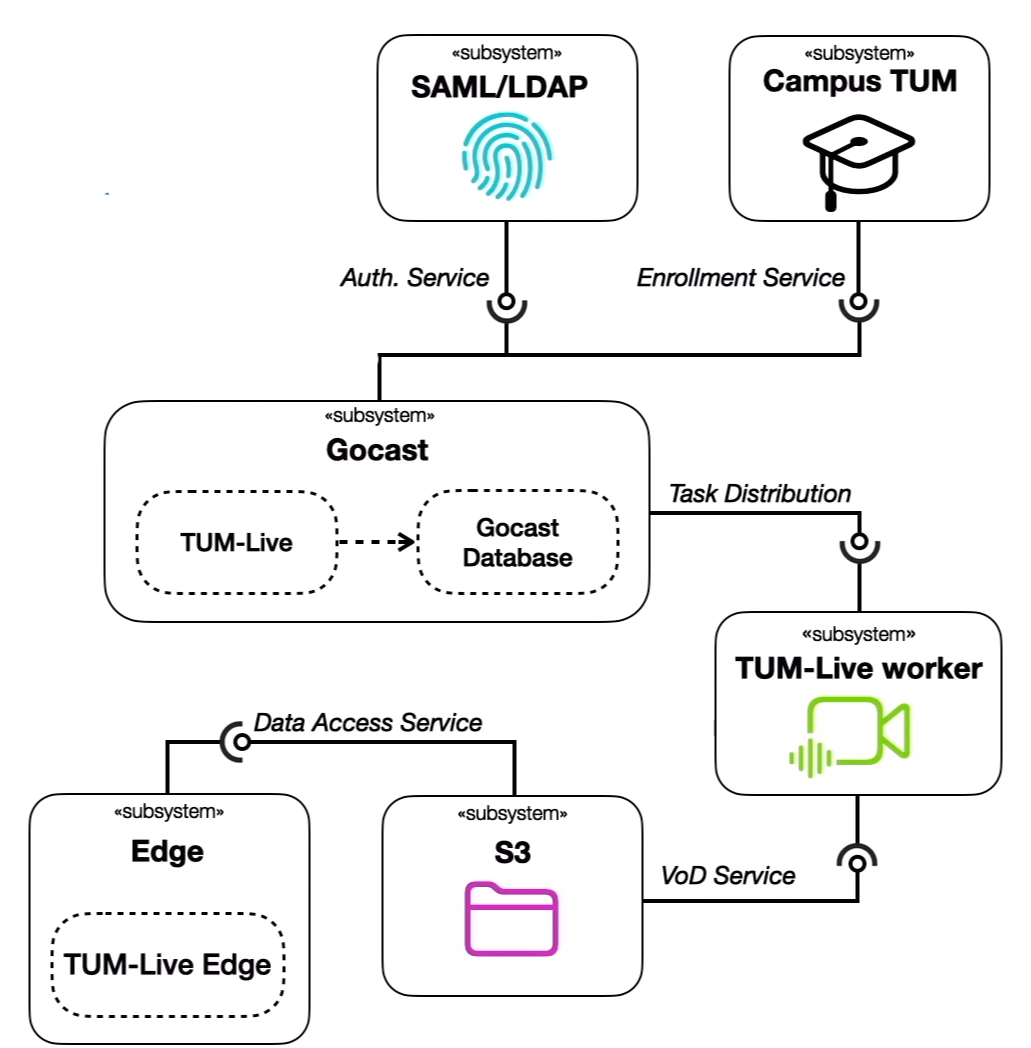
\includegraphics[width=\textwidth]{images/OldDeploymentDiagram.png}
    \caption[Subsystem Decomposition]{Subsystem Decomposition Model of TUM-Live}\label{fig:system-architecture}
\end{figure}

\subsection{Target System Architecture}

To distribute GoCast to different faculties, the subsystems and components responsible for processing and handling video data need to be distributed and hosted by each individual school. 
The main Tum-Live API instance however, will remain managed by the \ac{ITO} or TUM so that users have a single point of access (instead of having to switch instances when wanting to watch lectures of different faculties).
To achieve this, each faculty needs to host at least three components: the Runner / Worker component, the VoD service component and a Edge Server. 
Each school can then decide how many resources it wants to allocate to each service depending on their expected usage. The following minimum hardware requirements are set:

\begin{itemize}
    \item At least 1 VM as an Edge server. This server serves the videos to the users. Network throughput is important, so if a school serves many users, more instances are needed.
    \item At least 1 Worker or Runner VM. This server produces the stream, transcodes the VoD and much more. CPU performance is important here. On the same node, for every worker a VoD Service needs to be deployed to expose a simple HTTP interface that accepts file uploads and packages them to a HLS stream in a configured location. This stream may then be distributed by the Edge Server.
    \item Optionally, a school can add additional VMs for monitoring (grafana, prometheus, influx...) or for services such as the Voice Service for subtitling live streams and VoDs which requiring a NVIDIA CUDA equipped Server to transcribes streams using the Whisper LLM).
\end{itemize}

\begin{figure}[htpb]
    \centering
    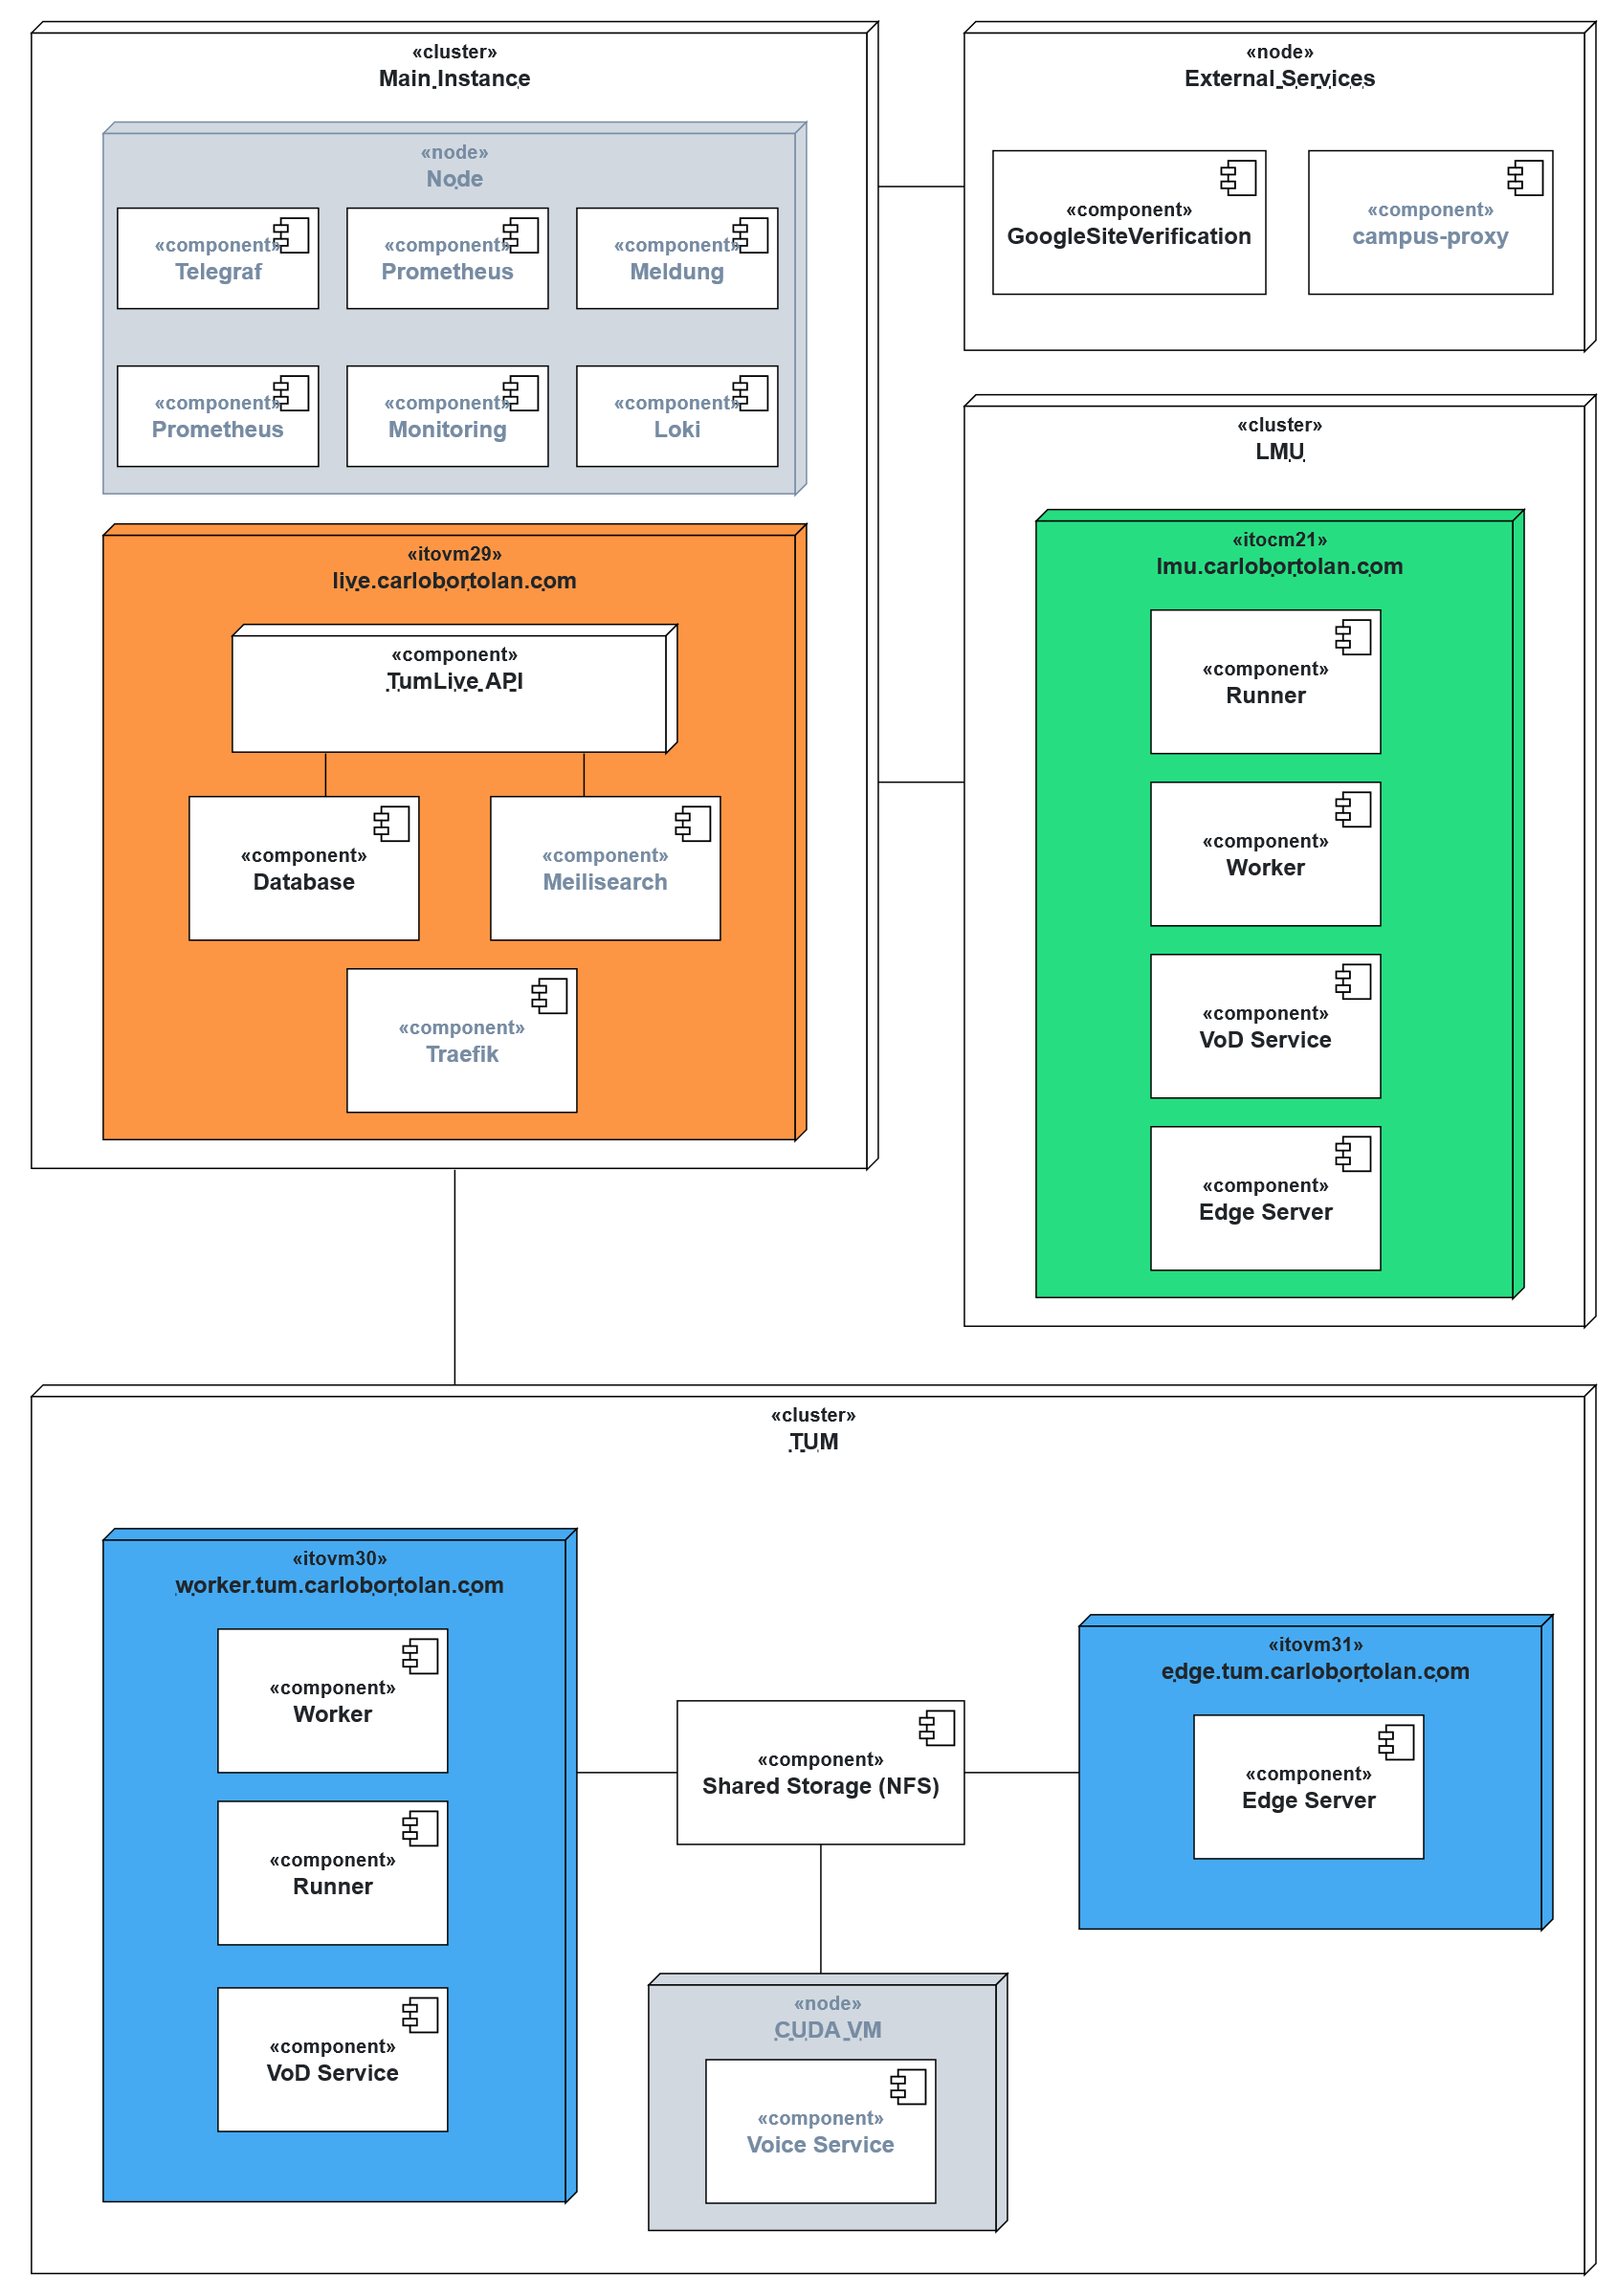
\includegraphics[width=\textwidth]{images/DeploymentDiagram.png}
    \caption[Target System Architecture]{Target Deployment Diagram of TUM-Live}\label{fig:system-architecture}
\end{figure}

\newpage

\subsection{Stats and Metrics of TUM-Live}

Since its creation in February of 2021, GoCast has been used to stream thousands of hours of video every semester for more than 150 courses and 15.000 Students. The source code is open-source, accessible at \href{https://github.com/TUM-Dev/gocast}{github.com/TUM-Dev/gocast} and licensed under the MIT license.

\section{Process, preparation, methods and environments}

The thesis spanned 5 months, from 15.05.2024 to \getSubmissionDate{}. The first weeks were spent familiarizing with the current system considering different approaches to scale its architecture and finding potential bottlenecks or issues. Following the initial analysis of the system, before being able to try scaling individual components, the original user and role system first needed to be updated together with new database models. After that, the most important components were gradually updated to be usable and manageable by each faculty. 
To develop and test the prototype of a distributed architecture for TUM-Live for this thesis, the following resources were used:
\begin{itemize}
    \item 3 \ac{VM}s with: 2 GB RAM, Intel(R) Xeon(R) CPU E5-2697A v4 @ 2.60GHz
    \item 1 \ac{VM} with: 20 GB RAM, AMD EPYC 7452 32-Core Processor
    \item 1 \ac{AWS} \ac{EKS} Cluster
    \item 1 selfhosted \ac{VM} with 32 GB RAM, AMD Ryzen 7 PRO 6850U @ 2.70GHz
\end{itemize}

After the target architecture had been deployed (on a smaller scale) using given resources, a set of performance tests and comparisons was made to find potential limits and breakpoints of each component. 
Additionally, in parallel to the development of the new architecture, a dedicated documentation has been created to facilitate the set up of GoCast for lecturers or new faculties which can be found at \href{https://tumlive-docs.pages.dev/}{tumlive-docs.pages.dev}. The documentation was created using Meta Opensource's Docusaurus. Static pages were deployed using Cloudflare.
All relevant source code for the thesis, new architecture, other mentioned prototypes and documentation can also be found at \href{https://github.com/carlobortolan/thesis}{github.com/carlobortolan/thesis}.

\section{Implementation Outline}

\subsection{Updating Architecture and Core API}

\subsection{Scaling Workers and Runners}

\subsection{Scaling Proxies and Other Services}

\subsection{Optimizing selected services}
